\documentclass[border=10pt]{standalone}
\usepackage{tikz}

\begin{document}

% z-y��-x�� (intrinsic rotations) or x-y-z (extrinsic rotations): the intrinsic rotations are known as: yaw, pitch and roll


% intrinsic rotation

% z psi
\begin{tikzpicture}
    \coordinate (o) at (0,0);
    
    \coordinate (x) at (-2,0);
    \coordinate (y) at (1.4,-1.4);
    \coordinate (z) at (0,2);

    \draw [->] (o) -- (x) node[left] {$x$};
    \draw [->] (o) -- (y) node[right] {$y$};
    % \draw [->] (o) -- (z) node[above] {$z$};
    
    \coordinate (x') at (-1.7,-.6);
    \coordinate (y') at (1.7,-.7);
    \coordinate (z') at (0,2);

    \draw [blue,->] (o) -- (x') node[left] {$x'$};
    \draw [blue,->] (o) -- (y') node[right] {$y'$};
    \draw [blue,->] (o) -- (z') node[above] {$z'(z)$};
    
    
    % psi x start
    \coordinate (pxs) at (-.5,0);
    \coordinate (pys) at (.35,-.35);
    % psi x label
    \coordinate (pxl) at (-.5,-.1);
    \coordinate (pyl) at (.35,-.35);
    
    \draw (pxs) arc [x radius=.5, y radius=.5, start angle=180, end angle=200];
    \draw (pys) arc [x radius=.35, y radius=.35, start angle=-45, end angle=-12];
    
    \node [left,font=\fontsize{6}{6}] at (pxl) {$\psi$};
    \node [right,font=\fontsize{6}{6}] at (pyl) {$\psi$};
 
\end{tikzpicture}

% y' theta
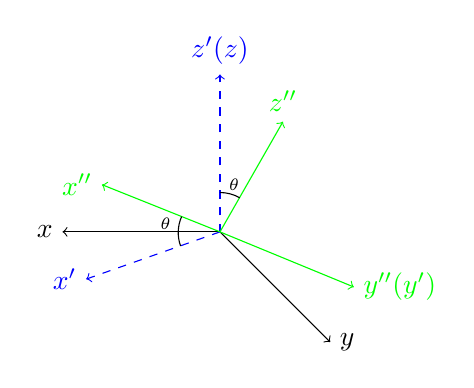
\begin{tikzpicture}
    \coordinate (o) at (0,0);
    
    \coordinate (x) at (-2,0);
    \coordinate (y) at (1.4,-1.4);
    \coordinate (z) at (0,2);

    \draw [->] (o) -- (x) node[left] {$x$};
    \draw [->] (o) -- (y) node[right] {$y$};
    % \draw [->] (o) -- (z) node[above] {$z$};
    
    \coordinate (x') at (-1.7,-.6);
    \coordinate (y') at (1.7,-.7);
    \coordinate (z') at (0,2);

    \draw [dashed,blue,->] (o) -- (x') node[left] {$x'$};
    % \draw [dashed,blue,->] (o) -- (y') node[right] {$y'$};
    \draw [dashed,blue,->] (o) -- (z') node[above] {$z'(z)$};
    
    
    \coordinate (x'') at (-1.5,.6);
    \coordinate (y'') at (1.7,-.7);
    \coordinate (z'') at (.8,1.4);
    
    \draw [green,->] (o) -- (x'') node[left] {$x''$};
    \draw [green,->] (o) -- (y'') node[right] {$y''(y')$};
    \draw [green,->] (o) -- (z'') node[above] {$z''$};
    
    
    
    % theta x start
    \coordinate (txs) at (-.5,-.18);
    \coordinate (tzs) at (0,.5);
    % theta x label
    \coordinate (txl) at (-.5,.1);
    \coordinate (tzl) at (.18,.4);
    
    \draw (txs) arc [x radius=.5, y radius=.5, start angle=200, end angle=156];
    \draw (tzs) arc [x radius=.5, y radius=.5, start angle=90, end angle=60];
    
    \node [left,font=\fontsize{6}{6}] at (txl) {$\theta$};
    \node [above,font=\fontsize{6}{6}] at (tzl) {$\theta$};
    
\end{tikzpicture}

% x'' phi
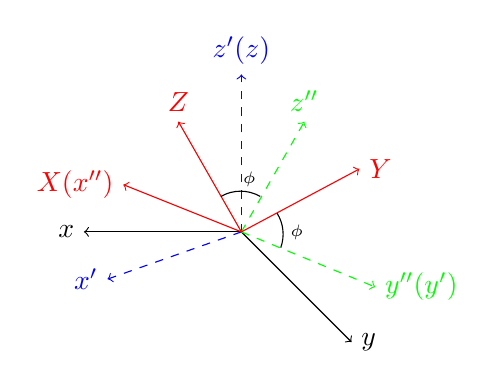
\begin{tikzpicture}
    \coordinate (o) at (0,0);
    
    \coordinate (x) at (-2,0);
    \coordinate (y) at (1.4,-1.4);
    \coordinate (z) at (0,2);

    \draw [->] (o) -- (x) node[left] {$x$};
    \draw [->] (o) -- (y) node[right] {$y$};
    % \draw [->] (o) -- (z) node[above] {$z$};
    
    \coordinate (x') at (-1.7,-.6);
    \coordinate (y') at (1.7,-.7);
    \coordinate (z') at (0,2);

    \draw [dashed,blue,->] (o) -- (x') node[left] {$x'$};
    % \draw [dashed,blue,->] (o) -- (y') node[right] {$y'$};
    \draw [dashed,blue,->] (o) -- (z') node[above] {$z'(z)$};
    
    
    \coordinate (x'') at (-1.5,.6);
    \coordinate (y'') at (1.7,-.7);
    \coordinate (z'') at (.8,1.4);
    
    % \draw [green,->] (o) -- (x'') node[left] {$x''$};
    \draw [dashed,green,->] (o) -- (y'') node[right] {$y''(y')$};
    \draw [dashed,green,->] (o) -- (z'') node[above] {$z''$};
    
    
    \coordinate (X) at (-1.5,.6);
    \coordinate (Y) at (1.5,.8);
    \coordinate (Z) at (-.8,1.4);
    
    \draw [red,->] (o) -- (X) node[left] {$X(x'')$};
    \draw [red,->] (o) -- (Y) node[right] {$Y$};
    \draw [red,->] (o) -- (Z) node[above] {$Z$};
    
    
    
    % phi x start
    \coordinate (phys) at (.5,-.2);
    \coordinate (phzs) at (.24,.45);
    % phi x label
    \coordinate (phyl) at (.5,0);
    \coordinate (phzl) at (.1,.45);
    
    \draw (phys) arc [x radius=.5, y radius=.5, start angle=-20, end angle=32];
    \draw (phzs) arc [x radius=.5, y radius=.5, start angle=60, end angle=120];
    
    \node [right,font=\fontsize{6}{6}] at (phyl) {$\phi$};
    \node [above,font=\fontsize{6}{6}] at (phzl) {$\phi$};
    
\end{tikzpicture}

\end{document}
